\documentclass{article}

\usepackage[utf8]{inputenc}
\usepackage[T1]{fontenc}
\usepackage[francais]{babel}
\usepackage{setspace}
\usepackage{listings} 
\usepackage{hyperref}
\usepackage{amssymb}
\usepackage{graphicx}
\usepackage[nottoc]{tocbibind}

\begin{document}
\begin{titlepage}
\lstset{language=C}
\title{Analyse, Classification, Indexation des données}
\author{Axel CAMUS
\and
Nicolas ETCHEVERRY}
\date{Master 1 Informatique\\ Université de Bordeaux}
\maketitle
\end{titlepage}

\section{Exercice 1}

Le nuage de points obtenu avec les 4 vecteurs n'étant pas suffisamment représentatif pour séparer les classes et pouvoir en éliminer une. Nous avons choisi de tracer les gaussienne de chaque vecteur: x1(rouge), x2(vert), x3(noir), x4(bleu) pour chacune des dimensions.

\begin{figure}[h]
\centerline{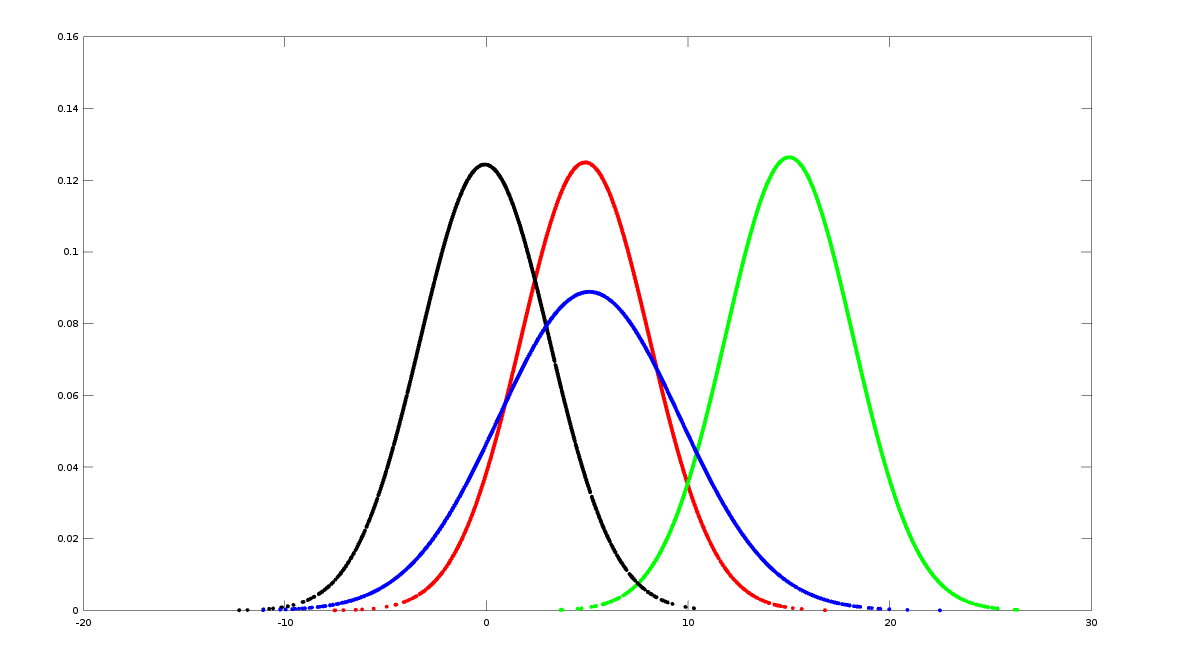
\includegraphics[scale=0.24]{donnee1.png}}
\caption{dimension 1}

\centerline{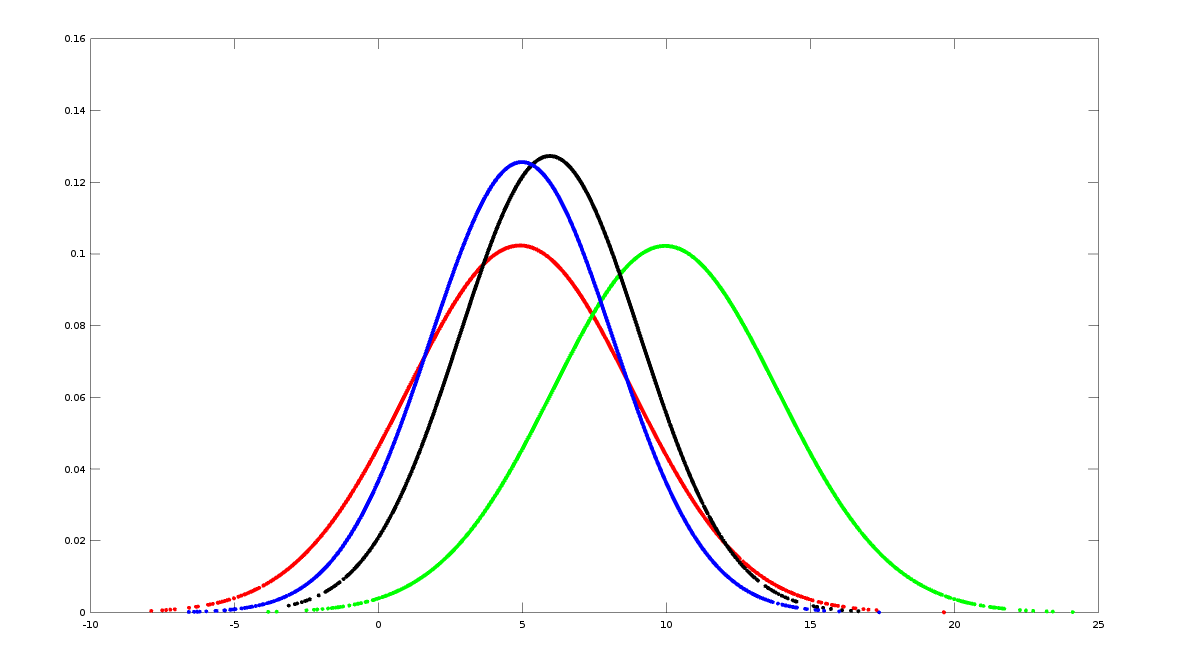
\includegraphics[scale=0.24]{donnee2.png}}
\caption{dimension 2}

\centerline{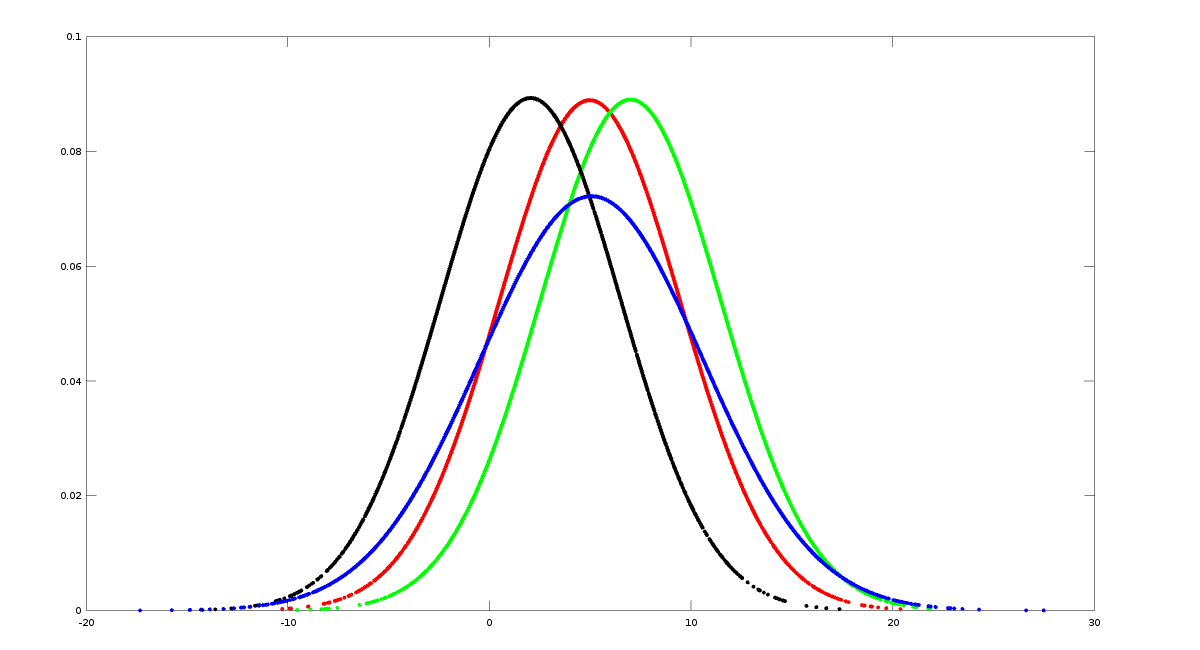
\includegraphics[scale=0.24]{donnee3.png}}
\caption{dimension 3}
\end{figure}

D'après les courbes précédente les données x1, x2 et x3 se démarquent plus les une des autres que les données x4. En choisissant ces 3 classes le classifieur donnera de meilleurs résultats qu'avec la classe 4 dont les données se perdent au milieu des autres classes.

\end{document}